\documentclass{article}

\usepackage{graphicx}
\usepackage{tikz}
\usepackage{tikzsymbols}
\usetikzlibrary{calc,patterns,shapes.geometric}
\pagestyle{empty}
\usepackage[margin=0pt]{geometry}
\geometry{papersize={14in,12in}}

\def\centerarc[#1](#2)(#3:#4:#5){\draw[#1] ($(#2)+({#5*cos(#3)},{#5*sin(#3)})$) arc (#3:#4:#5);}

\begin{document}
	\begin{figure}
		\centering
		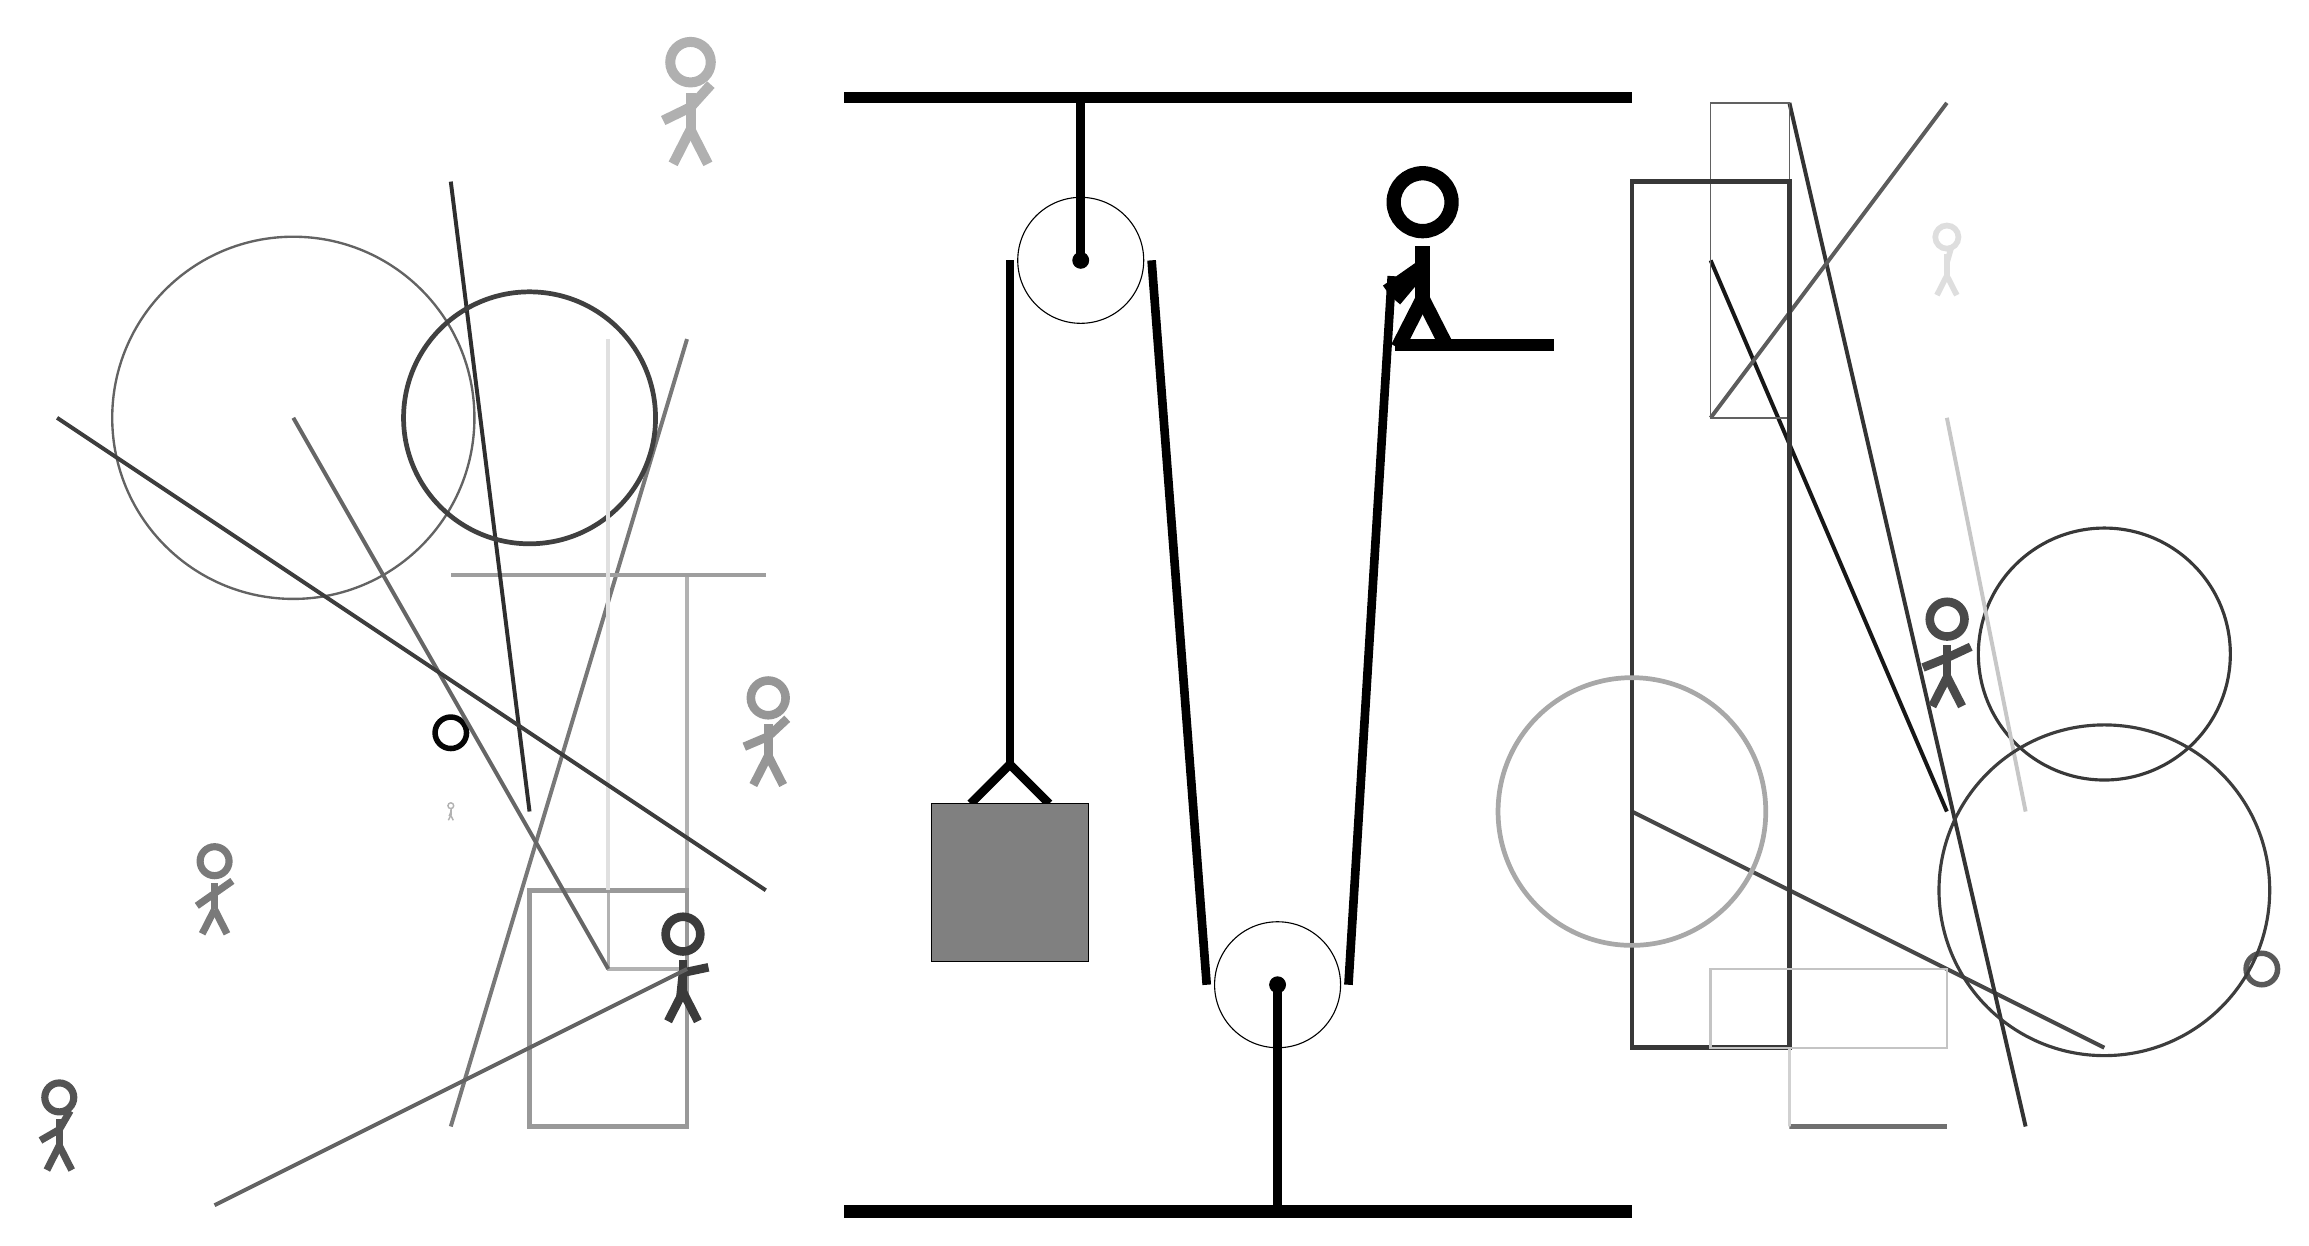
\begin{tikzpicture}
			%%%%% START %%%%%
			
			\draw[fill=black] (-2, 14) rectangle (8, 14.125);
			
			\draw (3.5, 2.8) circle (0.8);
			\draw[fill=black] (3.5, 2.8) circle (0.1);
			\draw[line width=1.1mm] (3.5, 2.8) -- (3.5, 0);
			
			\draw (1, 12) circle (0.8);
			\draw[fill=black] (1, 12) circle (0.1);
			\draw[line width=1.1mm] (1, 14) -- (1, 12);
			
			\draw[line width=1.1mm](-0.4, 5.1) --  (0.1, 5.6) -- (0.6, 5.1);
			\draw[fill=black!50] (-0.9, 5.1) rectangle (1.1, 3.1);
			
			\draw[line width=0.5mm, color=black!91](9, 12) -- (12, 5);
			
			\node[line width=0.4mm, color=black!13] at (12, 12) {\Strichmaxerl[4][90][74]};
			\node[line width=0.4mm, color=black!30] at (-7, 5) {\Strichmaxerl[1][67][83]};
			\draw[line width=0.5mm, color=black!72](8, 5) -- (14, 2);
			
			\draw [line width=0.4mm, color=black!78](14, 7) circle (1.6);
			\draw[line width=0.5mm, color=black!53](-4, 11) -- (-7, 1);
			
			\draw[line width=0.5mm, color=black!22](13, 5) -- (12, 10);
			\draw[line width=0.5mm, color=black!60] (9, 0) rectangle (9, 0);
			\draw[line width=0.4mm, color=black!30] (-4, 8) rectangle (-5, 3);
			\draw[line width=0.5mm, color=black!80](10, 14) -- (13, 1);
			\draw[line width=0.5mm, color=black!38](-3, 8) -- (-7, 8);
			
			\draw [line width=0.3mm, color=black!61](-9, 10) circle (2.3);
			\draw[line width=0.5mm, color=black!82](-7, 13) -- (-6, 5);
			
			\draw [line width=0.7mm, color=black!98](-7, 6) circle (0.2);
			\draw[line width=0.5mm, color=black!64](12, 14) -- (9, 10);
			\node[line width=0.3mm, color=black!31] at (-4, 14) {\Strichmaxerl[7][26][48]};
			
			\draw[line width=0.2mm, color=black!62] (10, 14) rectangle (9, 10);
			\draw[line width=0.6mm, color=black!40] (-4, 1) rectangle (-6, 4);
			\node[line width=0.3mm, color=black!77] at (-4, 3) {\Strichmaxerl[6][84][12]};
			\draw[line width=0.6mm, color=black!56] (10, 1) rectangle (12, 1);
			\draw [line width=0.7mm, color=black!65](16, 3) circle (0.2);
			\draw[line width=0.5mm, color=black!60](-5, 3) -- (-9, 10);
			\draw [line width=0.6mm, color=black!75](-6, 10) circle (1.6);
			\draw[line width=0.6mm, color=black!78] (10, 2) rectangle (8, 13);
			\draw[line width=0.3mm, color=black!18] (10, 1) rectangle (10, 2);
			\draw[line width=0.5mm, color=black!12](-5, 11) -- (-5, 4);
			\node[line width=0.7mm, color=black!67] at (-12, 1) {\Strichmaxerl[5][30][60]};
			\node[line width=0.4mm, color=black!71] at (12, 7) {\Strichmaxerl[6][22][25]};
			\draw[line width=0.5mm, color=black!61](-4, 3) -- (-10, 0);
			\node[line width=0.6mm, color=black!41] at (-3, 6) {\Strichmaxerl[6][23][43]};
			\draw [line width=0.6mm, color=black!34](8, 5) circle (1.7);
			
			\draw[line width=0.5mm, color=black!76](-3, 4) -- (-12, 10);
			\draw[line width=0.3mm, color=black!23] (9, 2) rectangle (12, 3);
			\draw [line width=0.4mm, color=black!76](14, 4) circle (2.1);
			\node[line width=0.7mm, color=black!52] at (-10, 4) {\Strichmaxerl[5][35][35]};
			
			\draw[line width=1.1mm](0.1, 12) -- (0.1, 5.6);
			\centerarc[line width=1.1mm](1, 12)(180:0:0.9)
			\draw[line width=1.1mm](1.9, 12) -- (2.6, 2.8);
			\centerarc[line width=1.1mm](3.5, 2.8)(180:360:0.9)
			\draw[line width=1.1mm](4.4, 2.8) -- (4.95, 11.8);
			
			\node at (5.3, 12) {\Strichmaxerl[10][35][-130]};
			\draw[fill=black] (5, 11) rectangle (7, 10.85);
			
			\draw[fill=black] (-2, 0) rectangle (8, -0.15);
			
			%%%%% END %%%%%
		\end{tikzpicture}
	\end{figure}	
\end{document}